\documentclass[11pt]{beamer}

\usetheme[sectionpages,logo={_figures/poli-blue.pdf}]{UniNA}
\usefonttheme[onlymath]{serif}

\usepackage{tikz}
\usepackage{graphicx}
\usepackage{caption}
\usepackage{subcaption}
\usepackage{stanli}
\usepackage{siunitx}
\usepackage{mathtools}
\usepackage{quotes}
\usepackage{amsmath}
\usepackage{empheq}

\title{Sistema de suspensão rocker-bogie} %shown in title frame
\subtitle{PEF-3208 - Fundamentos em Mecânica das Estruturas}  % could also be a conference name

\date{\today} %explicitly set date instead of \today

\author[Natanael M. Cardoso]{Natanael Magalhães Cardoso}

\institute{Escola Politécnica - Universidade de São Paulo}

\begin{document}

\maketitle

\section{Introdução}

\begin{frame}{Sobre o sistema rocker-bogie}
  \begin{columns}
    \column{.59\textwidth}
    \begin{itemize}
      \item Desenvolvido em 1988 para o uso da NASA na exploração de Marte.
      \item Usado para movimentar robôs de 6 rodas.
    \end{itemize}
    \column{.39\textwidth}
    \begin{figure}[ht]
      \centering
      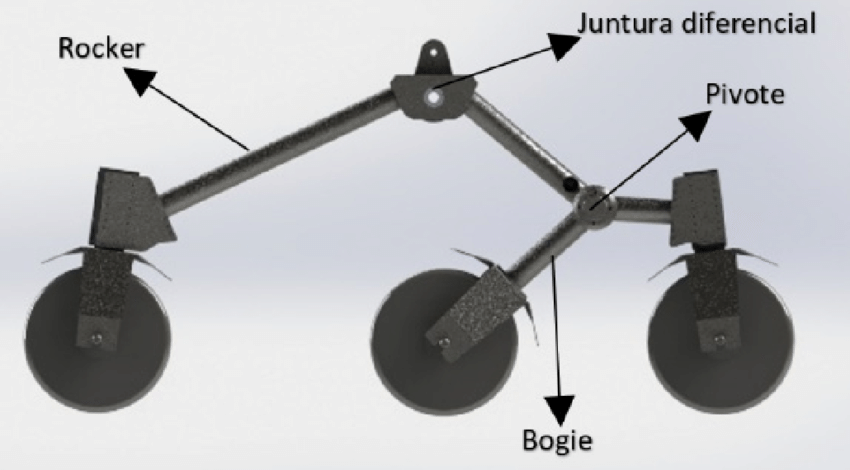
\includegraphics[width=.9\textwidth]{fig/rb-suspension.png}
    \end{figure}
    \vspace{5mm}
    \begin{figure}[ht]
      \centering
      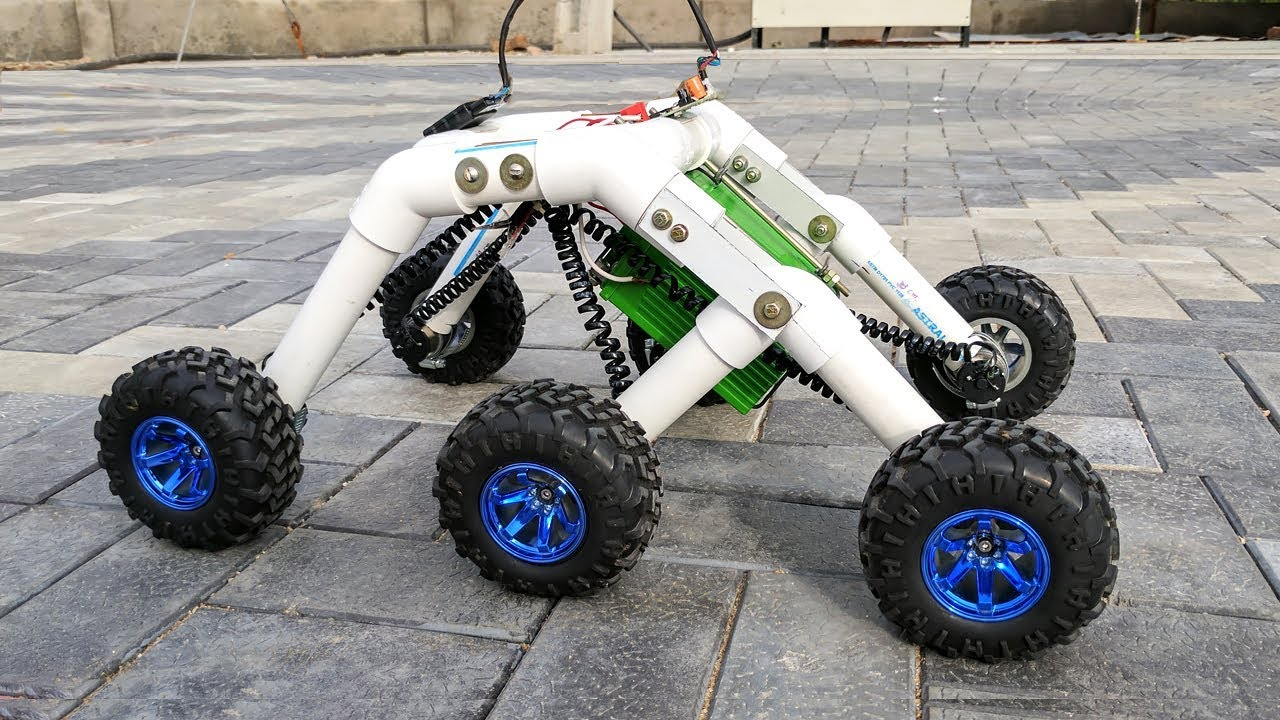
\includegraphics[width=.9\textwidth]{fig/rb.jpg}
    \end{figure}
  \end{columns}
\end{frame}

\begin{frame}{Uso do sistema de suspensão}
  % \vspace{12mm}
  \begin{figure}[ht]
    \begin{minipage}[b]{.32\textwidth}
      \centering
      Sojourner (1996)
      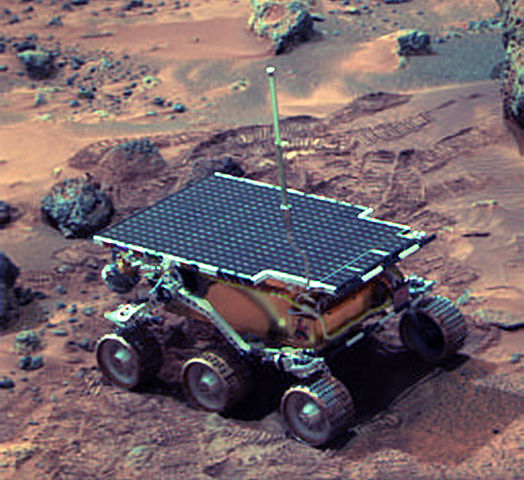
\includegraphics[width=.9\textwidth,height=2.8cm]{fig/sojourner.jpg}
    \end{minipage}%
    \begin{minipage}[b]{.32\textwidth}
      \centering
      Spirit (2003)
      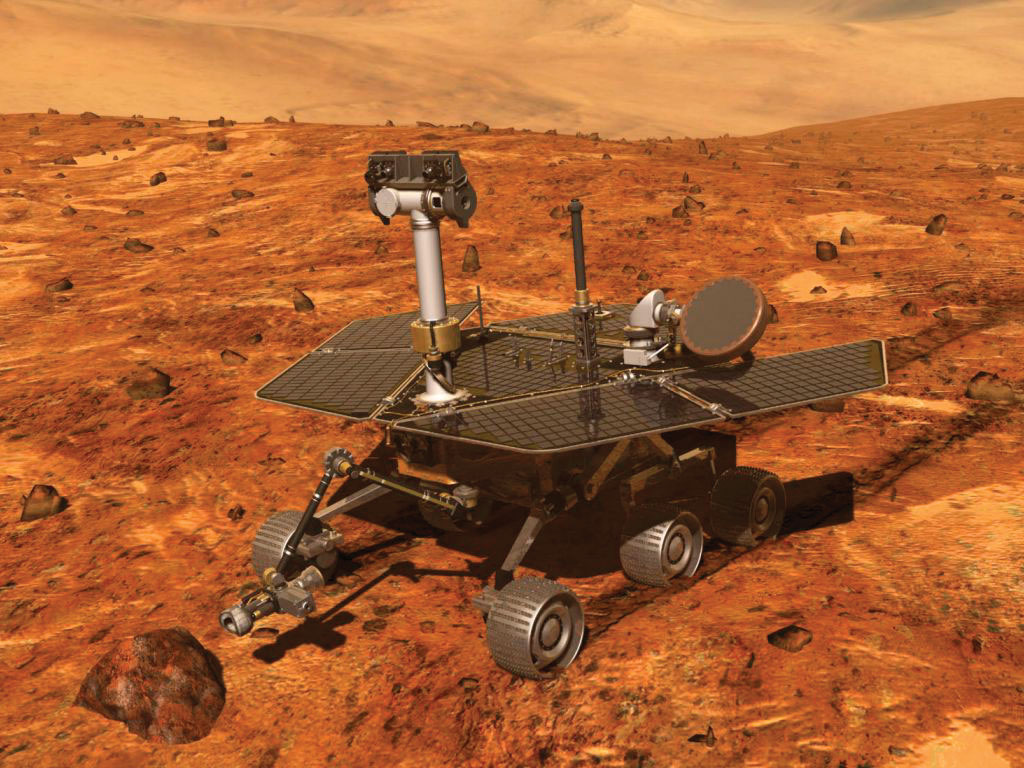
\includegraphics[width=.9\textwidth,height=2.8cm]{fig/spirit.jpg}
    \end{minipage}%
    \begin{minipage}[b]{.32\textwidth}
      \centering
      Opportunity (2003)
      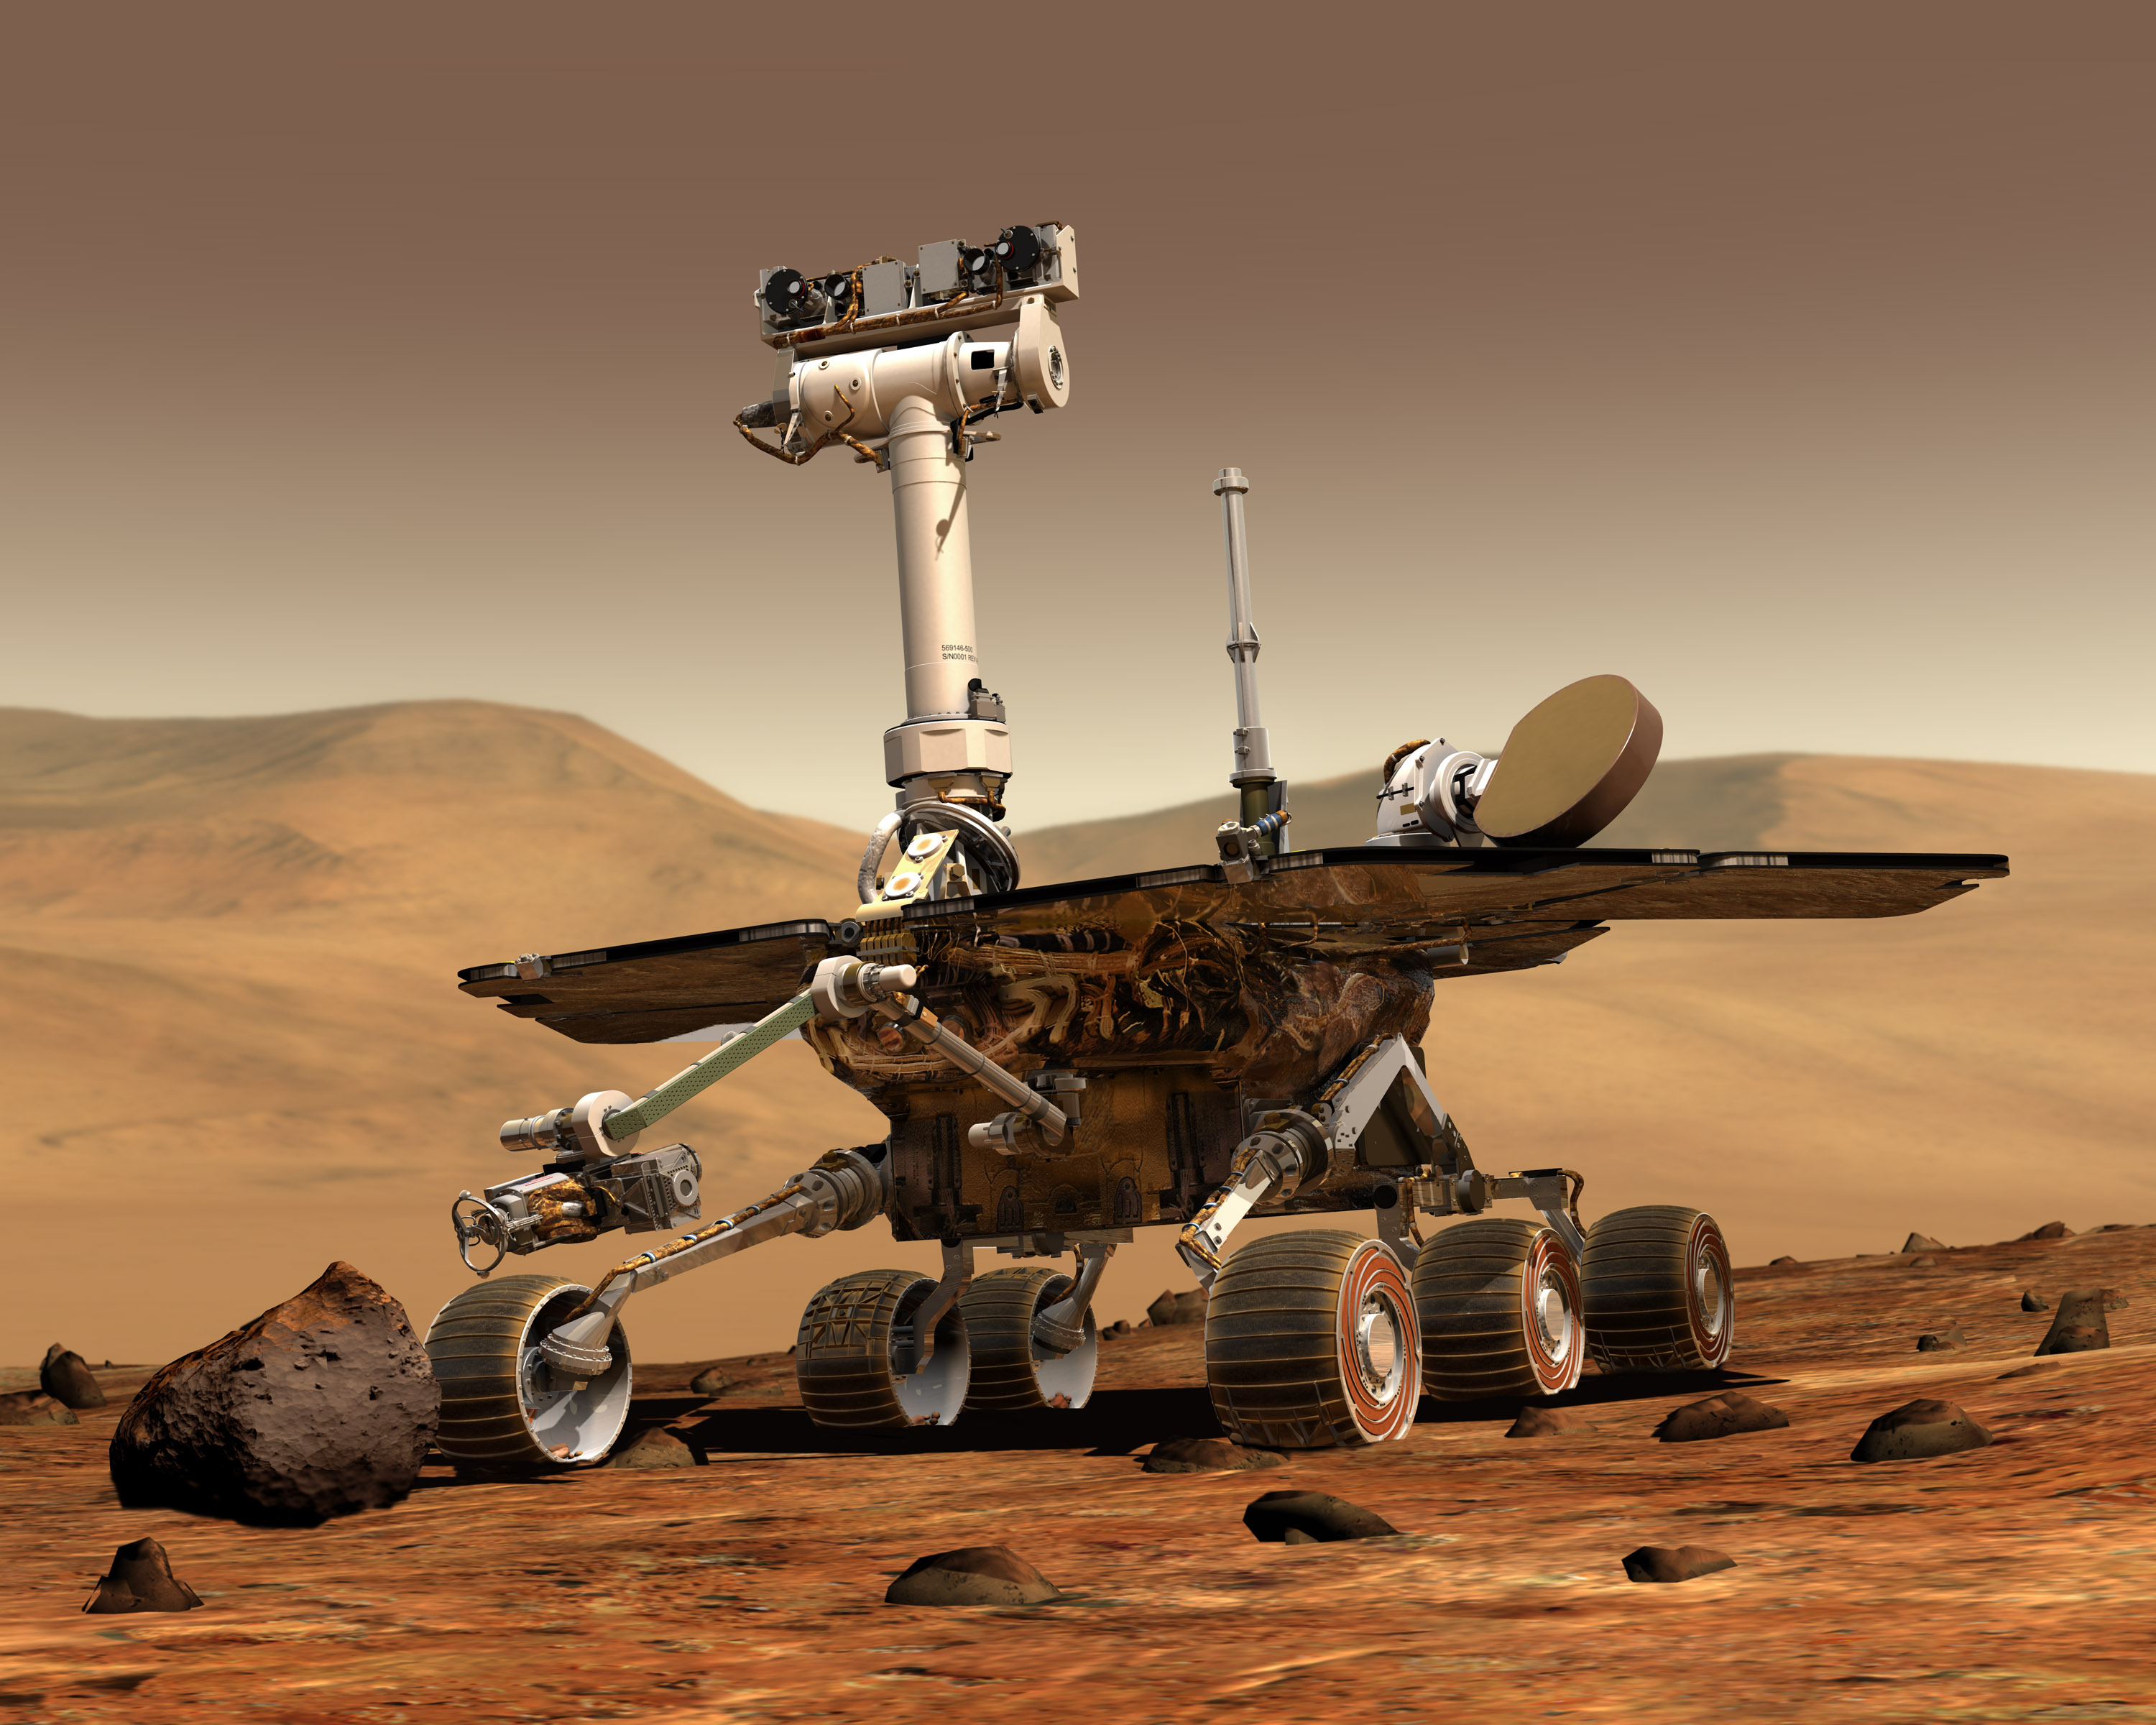
\includegraphics[width=.9\textwidth,height=2.8cm]{fig/opportunity.jpg}
    \end{minipage}
  \end{figure}
  \vspace{-4mm}
  \begin{figure}[ht]
    \begin{minipage}[b]{.32\textwidth}
      \centering
      Curiosity (2011)
      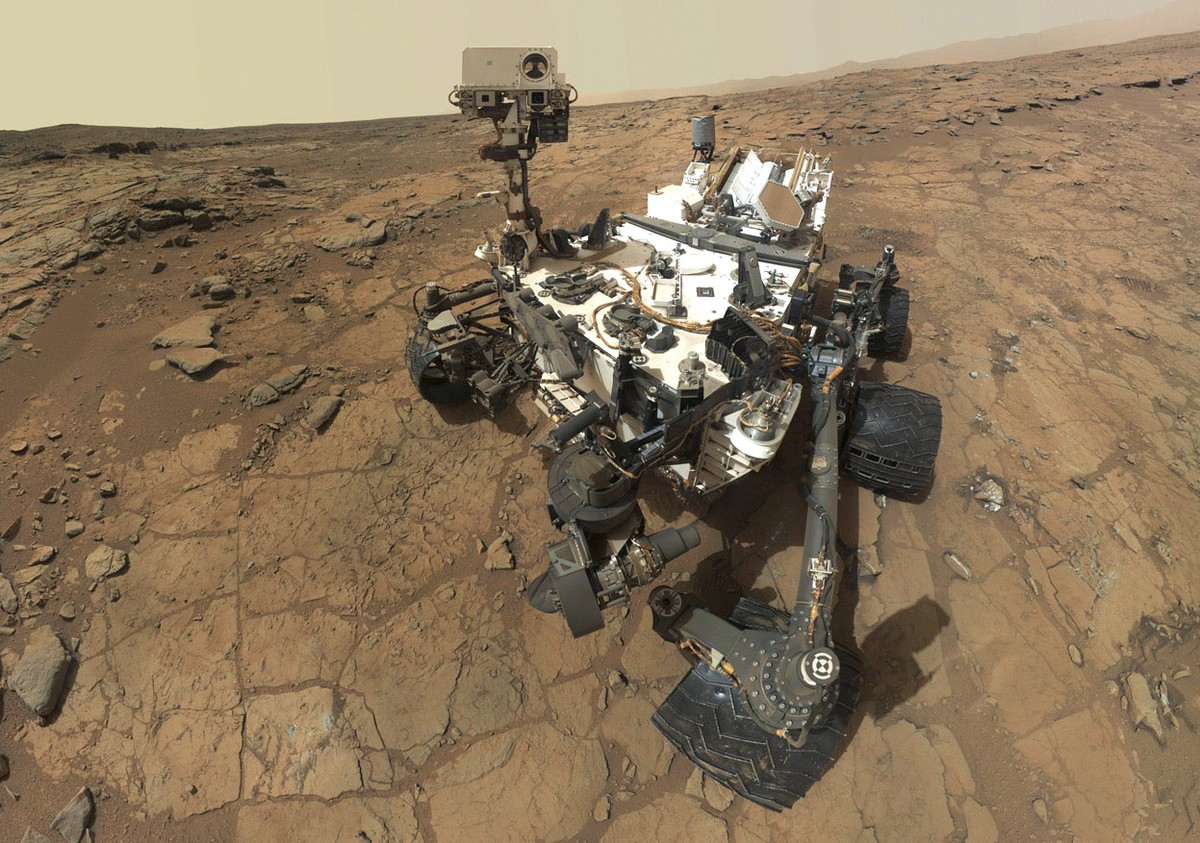
\includegraphics[width=.9\textwidth,height=2.8cm,trim={11cm 0 6.5cm 0},clip]{fig/curiosity.jpg}
    \end{minipage}%
    \hspace{5mm}
    \begin{minipage}[b]{.32\textwidth}
      \centering
      Perseverance (2020)
      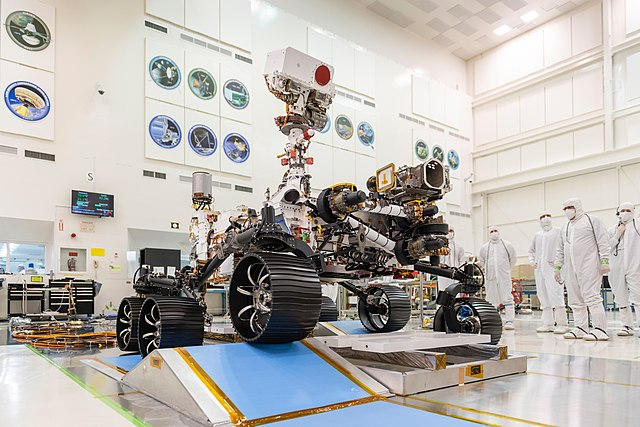
\includegraphics[width=.9\textwidth,height=2.8cm]{fig/perseverance.jpg}
    \end{minipage}%
  \end{figure}
\end{frame}

\section{Análise da Estrutura}

\begin{frame}{Diagrama da Estrutura}
  \begin{figure}[ht]
    \centering
    \resizebox{.8\textwidth}{!}{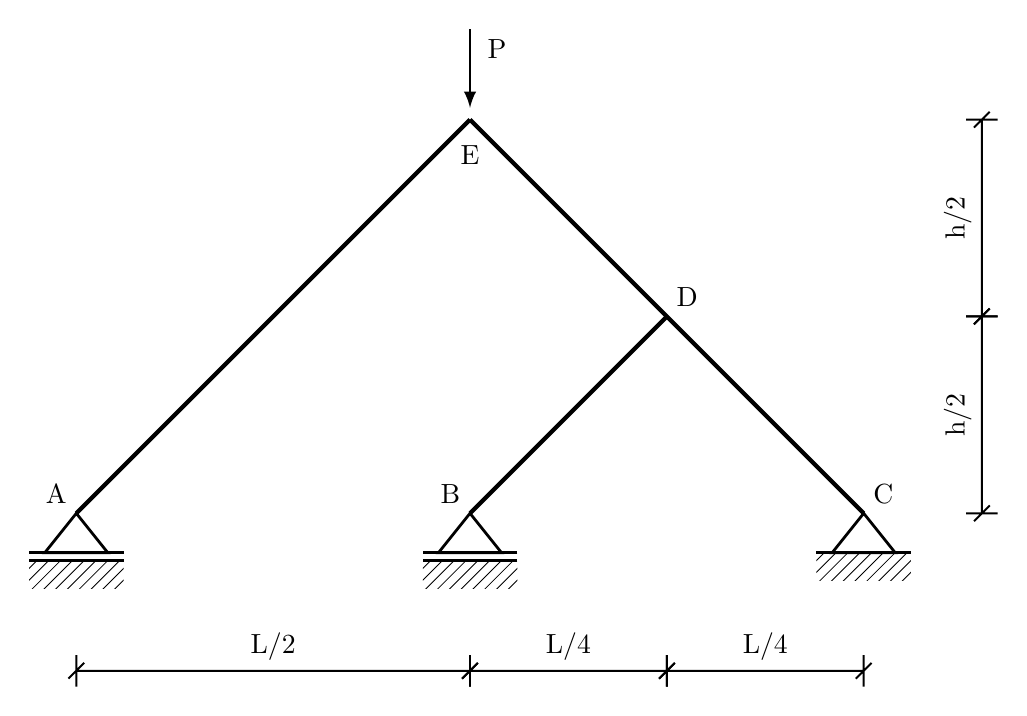
\begin{tikzpicture}
  \begin{scope}
    \point{a}{0}{0};
    \point{b}{5}{0};
    \point{c}{10}{0};
    \point{d}{7.5}{2.5};
    \point{e}{5}{5};

    \beam{2}{a}{e};
    \beam{2}{e}{c};
    \beam{2}{d}{b};

    \support{2}{a};
    \support{2}{b};
    \support{1}{c};

    \dimensioning{1}{a}{b}{-2}[L/2];
    \dimensioning{1}{b}{d}{-2}[L/4];
    \dimensioning{1}{d}{c}{-2}[L/4];
    \dimensioning{2}{d}{e}{11.5}[h/2];
    \dimensioning{2}{c}{d}{11.5}[h/2];

    \load{1}{e}[90];

    \dnotation{1}{e}{P}[yshift=9mm,right=1mm];
    \dnotation{1}{a}{A}[above left];
    \dnotation{1}{b}{B}[above left];
    \dnotation{1}{c}{C}[above right];
    \dnotation{1}{d}{D}[above right];
    \dnotation{1}{e}{E}[below=2mm];
  \end{scope}
\end{tikzpicture}}
  \end{figure}
\end{frame}

\begin{frame}{Simplificação}
  \begin{figure}[ht]
    \centering
    \resizebox{.8\textwidth}{!}{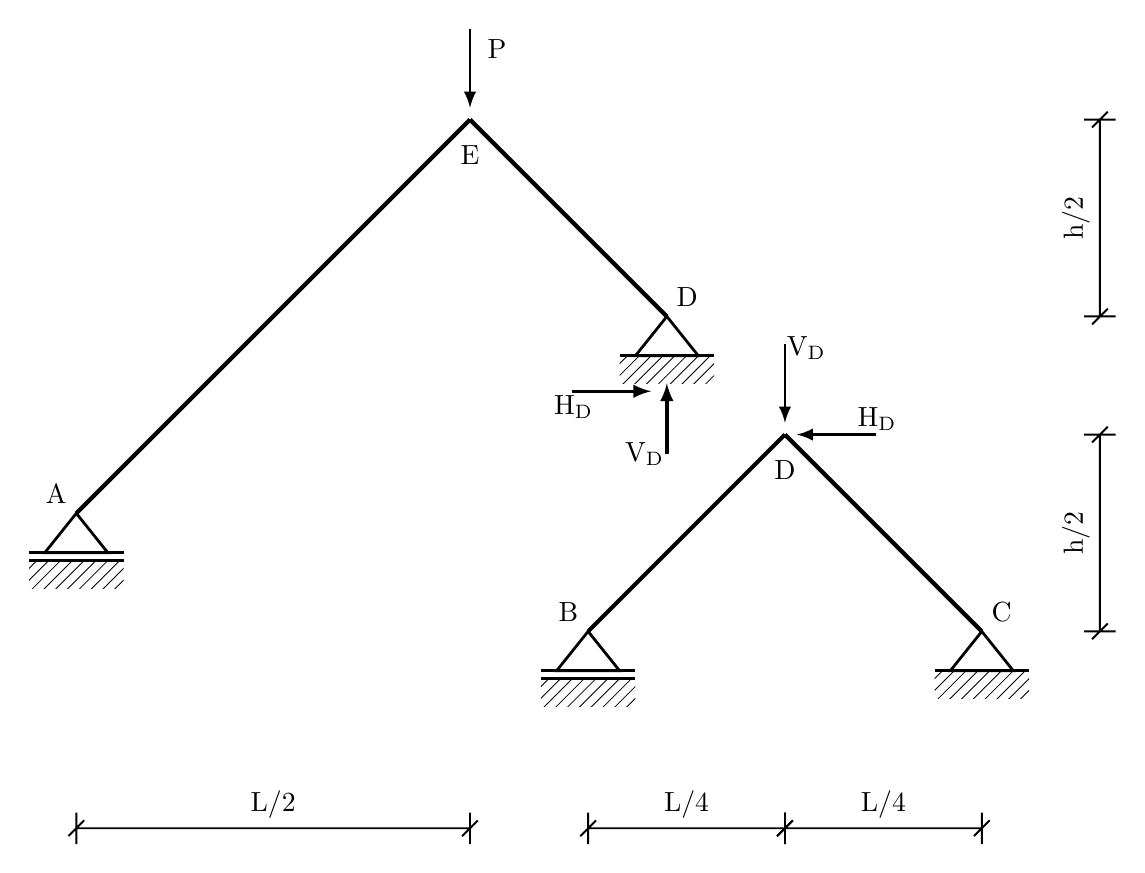
\begin{tikzpicture}
  \begin{scope}
    \point{a}{0}{0};
    \point{b}{6.5}{-1.5};
    \point{c}{11.5}{-1.5};
    \point{d1}{7.5}{2.5};
    \point{d2}{9}{1};
    \point{e}{5}{5};

    \beam{2}{a}{e};
    \beam{2}{d1}{e};
    \beam{2}{b}{d2};
    \beam{2}{c}{d2};

    \support{2}{a};
    \support{2}{b};
    \support{1}{c};
    \support{1}{d1};

    \dimensioning{1}{a}{e}{-4}[L/2];
    \dimensioning{1}{b}{d2}{-4}[L/4];
    \dimensioning{1}{d2}{c}{-4}[L/4];
    \dimensioning{2}{d1}{e}{13}[h/2];
    \dimensioning{2}{c}{d2}{13}[h/2];

    \load{1}{e}[90];

    \dnotation{1}{e}{P}[yshift=9mm,right=1mm];
    \dnotation{1}{a}{A}[above left];
    \dnotation{1}{b}{B}[above left];
    \dnotation{1}{c}{C}[above right];
    \dnotation{1}{d1}{D}[above right];
    \dnotation{1}{d2}{D}[below=2mm];
    \dnotation{1}{e}{E}[below=2mm];

    \draw[-{latex[scale=3.0]},very thick] (7.5,0.75) -- (7.5,1.65) node[yshift=-3mm,left=8mm] {H\textsubscript{D}};
    \draw[-{latex[scale=3.0]},very thick] (6.3,1.55) -- (7.3,1.55) node[yshift=-8mm,left=-3mm] {V\textsubscript{D}};
    \load{1}{d2}[90];
    \dnotation{1}{d2}{H\textsubscript{D}}[yshift=2mm,right=8mm];
    \load{1}{d2}[360];
    \dnotation{1}{d2}{V\textsubscript{D}}[yshift=11mm,right=-1mm];
  \end{scope}
\end{tikzpicture}}
  \end{figure}
\end{frame}

\begin{frame}{Análise da Primeira Estrutura}
  \begin{figure}[ht]
    \centering
    \resizebox{.75\textwidth}{!}{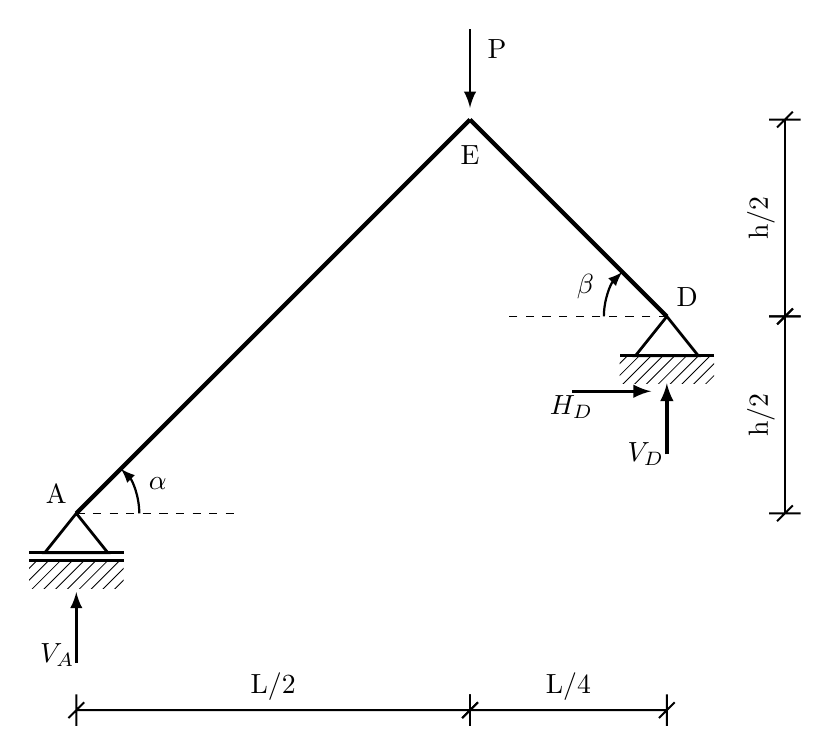
\begin{tikzpicture}
  \begin{scope}
    \point{a}{0}{0};
    \point{b}{6.5}{-1.5};
    \point{c}{11.5}{-1.5};
    \point{d1}{7.5}{2.5};
    \point{d2}{9}{1};
    \point{e}{5}{5};

    \beam{2}{a}{e};
    \beam{2}{d1}{e};

    \support{2}{a};
    \support{1}{d1};

    \dimensioning{1}{a}{e}{-2.5}[L/2];
    \dimensioning{1}{e}{d1}{-2.5}[L/4];
    \dimensioning{2}{a}{d1}{9}[h/2];
    \dimensioning{2}{d1}{e}{9}[h/2];

    \load{1}{e}[90];

    \dnotation{1}{e}{P}[yshift=9mm,right=1mm];
    \dnotation{1}{a}{A}[above left];
    \dnotation{1}{d1}{D}[above right];
    \dnotation{1}{e}{E}[below=2mm];

    \draw[-{latex[scale=3.0]},very thick] (7.5,0.75) -- (7.5,1.65) node[yshift=-3mm,left=8mm] {$H_D$};
    \draw[-{latex[scale=3.0]},very thick] (6.3,1.55) -- (7.3,1.55) node[yshift=-8mm,left=-3mm] {$V_D$};
    \load{1}{a}[270][.9][1];
    \dnotation{1}{a}{$V_A$}[left=-1mm,yshift=-18mm];

    \draw[-{latex[scale=3.0]},thick] (.8,0) arc (0:45:.8) node[] at (20:1.1) {$\alpha$};
    \draw[dashed] (0,0) -- (2,0);
    \draw[-{latex[scale=3.0]},thick] (6.7,2.5) arc (180:135:.8) node[shift=({7.5,2.5})] at (160:1.1) {$\beta$};
    \draw[dashed] (7.5,2.5) -- (5.5,2.5);
  \end{scope}
\end{tikzpicture}}
  \end{figure}
\end{frame}

\end{document}